\documentclass[simplex.tex]{subfiles}
% NO NEED TO INPUT PREAMBLES HERE
% packages are inherited; you can compile this on its own

\onlyinsubfile{
\title{NeuroData SIMPLEX Report: Subfile}
}

\begin{document}
\onlyinsubfile{
\maketitle
\thispagestyle{empty}

The following report documents the progress made by the labs of Randal~Burns and Joshua~T.~Vogelstein at Johns Hopkins University towards goals set by the DARPA SIMPLEX grant.

%%%% Table of Contents
\tableofcontents

%%%% Publications
\bibliographystyle{IEEEtran}
\begin{spacing}{0.5}
\section*{Publications, Presentations, and Talks}
\vspace{-20pt}
\nocite{*}
{\footnotesize	\bibliography{simplex}}
\end{spacing}
%%%% End Publications
}

\subsection{Science in the Cloud (SIC)}

Science in the cloud~(SIC) is an extensibility-focused scientific framework which addresses universal
challenges in the computational sciences. Currently, re-performing and extending published analyses
whether through new data or code is often unbearably difficult; (i) data may be closed-access; (ii) data 
may be organized in an ad hoc fashion; (iii) the code may be closed-source or undocumented; (iv) code may
have been run with undocumented parameters and dependencies; (v) analyses may have run with specifically
hardware compiled code. These properties make validating and extending scientific claims challenging.

We propose a solution to these gaps in the form of a framework which leverages publicly documented and deployable
cloud instances with specific pipelines installed and configured to extend published findings; an implementation we
simply term ''science in the cloud,'' or, SIC~(Latin for ''thus was it written'').
To address data access, we put data in the cloud.
To address data organization, we utilize recently proposed data standards.
To address closed source and undocumented, we generate open-source code and interactive demonstrations.
To address software and hardware dependencies, we utilize virtualization, automated deployment, and cloud computing.
SIC puts these pieces together to create a computing instance launched in the cloud designed for not only
producing reproducible research, but enabling easily accessible and extensible science for everyone. SIC is designed
to minimize the bottlenecks between publication and novel discoveries; leveraging the experience of the community,
we propose a solution for transitioning to a universal, and ''future-proof,'' deployment of software to the cloud.

A live demonstration is available at \href{http://scienceinthe.cloud}{http://scienceinthe.cloud}, which illustrates
this framework. There are six key components which much be considered in sic: data storage, data organization,
interactive demos, virtualization, computing, and deployment. The selection made for each of these components
will have a significant impact on available selections for the others. The final product will be a highly
interdependent network of tools and data.

\begin{figure}[h!]
\begin{cframed}
\centering
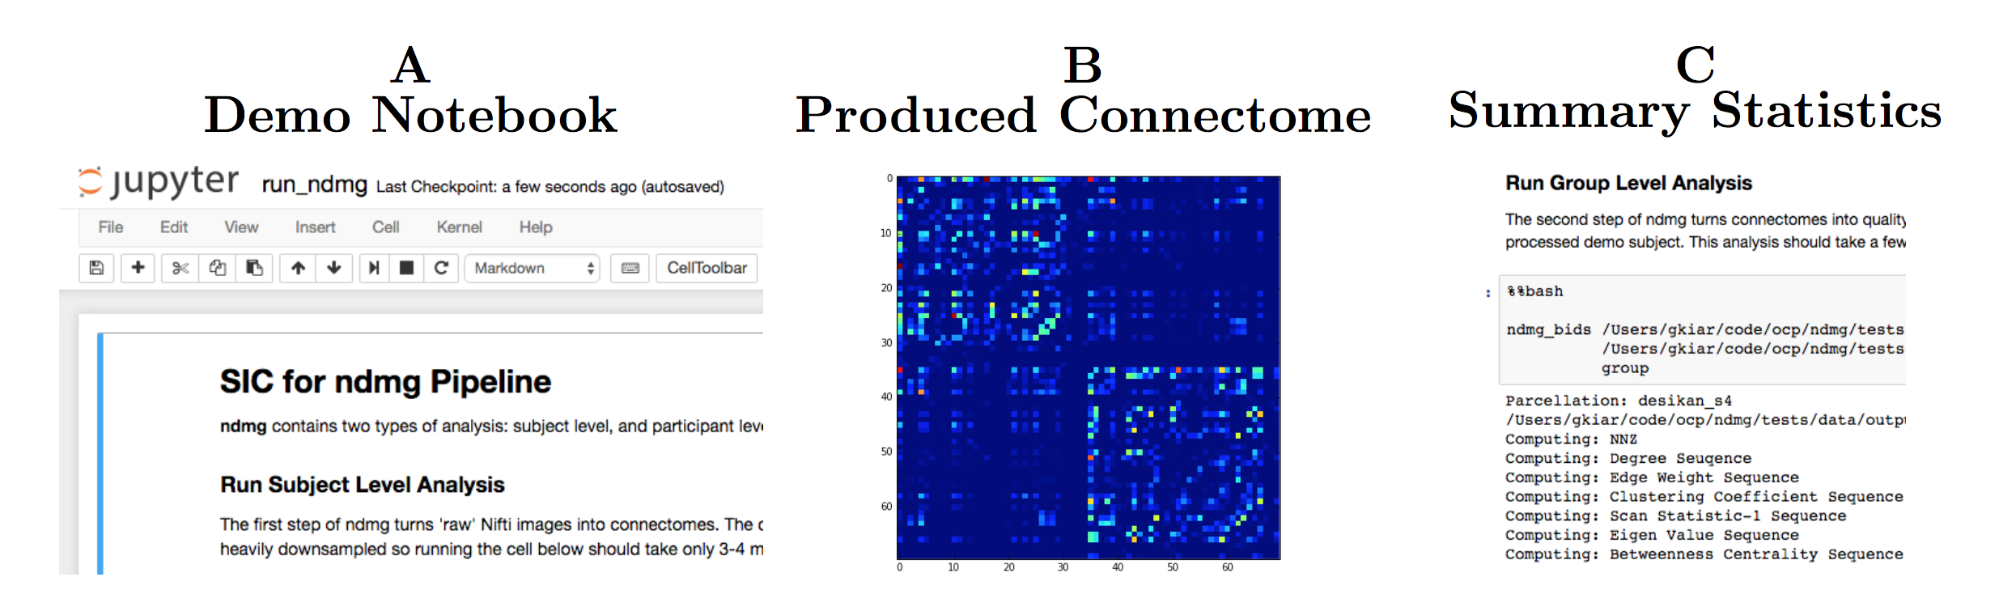
\includegraphics[width=0.95\textwidth]{./figs/sic.png}
\caption{
  States of the demo notebook in the cloud. A) A Jupyter notebook
  displaying descriptions and code snippets to be run for both
  connectome estimation and summary statistic computation. B) After
  running connectome generation an adjacency matrix will appear to
  provide a visualization. C) Summary statistic computation calculates
  several graph features and plots them in a multipanel figure. 
}
\label{fig:sic}
\end{cframed}
\end{figure}

\begin{figure}[h!]
\begin{cframed}
\centering
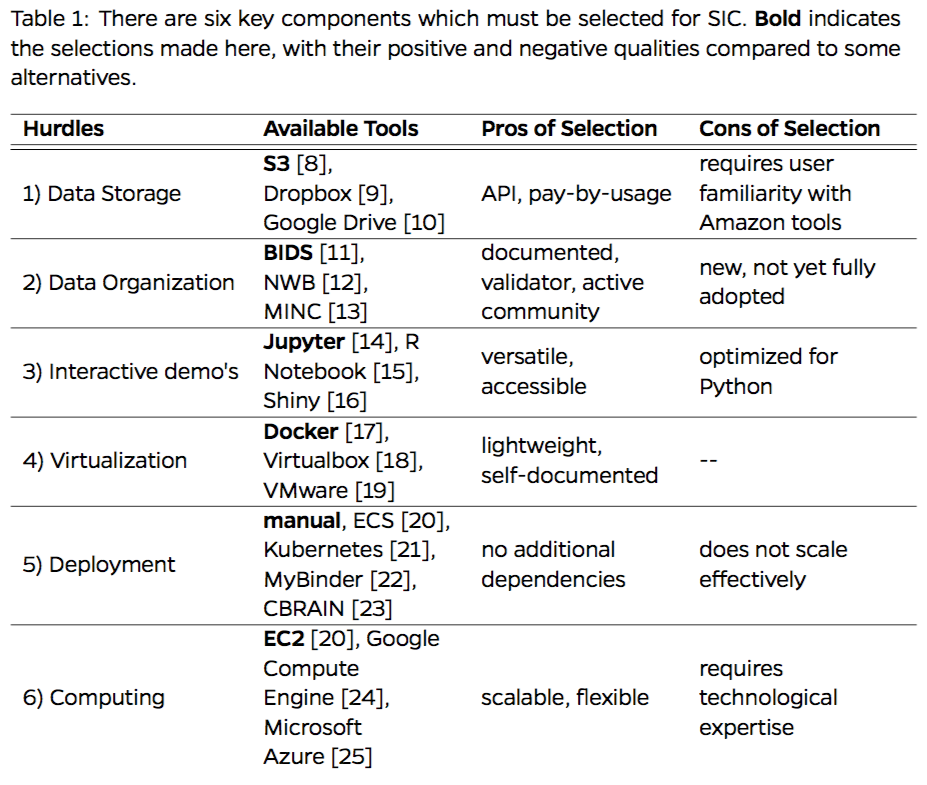
\includegraphics[width=0.85\textwidth]{./figs/sicTab.png}
\caption{
  Excerpted table from \cite{kiar2016}.
}
\label{fig:sicTab}
\end{cframed}
\end{figure}
\end{document}
